\chapter{Research Plan}
\label{cha:research_plan}

As previously mentioned in Section~\ref{subsec:what_are_dna_sequences}, by looking at the sequence of a DNA segment, scientists can figure out what kind of genetic information it contains. 

Scientists can utilize sequence information to determine which stretches of DNA include genes and which stretches have regulatory instructions that turn genes on or off. This is achieved by finding a protein called \gls{TF} that, by binding to a specific \gls{DNA} sequence, regulates the pace at which genetic information is transferred from DNA to messenger RNA. \gls{TF}s control genes by turning them on and off so that they are expressed in the proper cells at the right time and in the right amount throughout the cell's and organism's lives. The research of \gls{TF} function begins with accurate identification of \gls{TF}s~\cite{Hu2019AnimalTFDBFactors}.

It is also possible to explore the sequence data to identify essential genes. These are a group of genes that are required for a living organism's survival or reproduction~\cite{Zhang2020DeepHE:Learning}. Several wet-lab experimental approaches can be used to identify essential genes, however these procedures are frequently time-consuming, arduous, and expensive. Some classic \gls{ML}-based approaches have been offered as a complement to the experimental methods, with the primary goal of predicting essential genes on model organisms~\cite{Zhang2020DeepHE:Learning}.

The main aim of this work is to develop an automatic classification system for DNA sequences using deep learning algorithms. Because current solutions for DNA sequence classification use sequence similarity, which is a slow and less accurate method, the proposed project is expected to improve the response time and accuracy of the classification process. Both transcription factors and essential genes will be used as case studies for the platform validation.

The work will address the following tasks:

\begin{itemize}
    \item \textbf{Task 1}: Review relevant literature, study and write the state-of-the-art and analyze available data and tools regarding both \gls{ML} and \gls{DL} methods and their applications in sequence classification. The outcome of this task is this pre-thesis report.
    \item \textbf{Task 2}: Evaluate different existing algorithms and tools for data pre-processing and \gls{ML}/\gls{DL} approaches for classifying DNA sequences. The available methods will be compared with each other in terms of the impact on the classification performance of the \gls{ML} and \gls{DL} models.
    \item \textbf{Task 3}: Developing \gls{ML}/\gls{DL} based tools for DNA sequence classification, integrating them into \textit{ProPythia}~\cite{Sequeira2020ProPythia:Learning}. As mentioned in Section~\ref{sec:context_and_motivation}, this tool is devoted to the classification of peptides and protein sequences using \gls{ML} and \gls{DL} and one of the objectives of this thesis is to integrate a tool that supports \gls{DNA} sequence classifiers into the mentioned platform.
    \item \textbf{Task 4}: Developing \gls{AutoML} classifiers for \gls{DNA} sequences and integrating them into \textit{OmniumAI} software platforms.
    \item \textbf{Task 5}: Validation and test of the tools and platform with selected case studies (transcription factor annotation and essential genes determination). 
    \item \textbf{Task 6}: Write the master thesis.
\end{itemize}

Figure~\ref{fig:gantt} provides an overview of the project schedule with all the tasks above mentioned.

\begin{figure}[htbp]
    \centering
    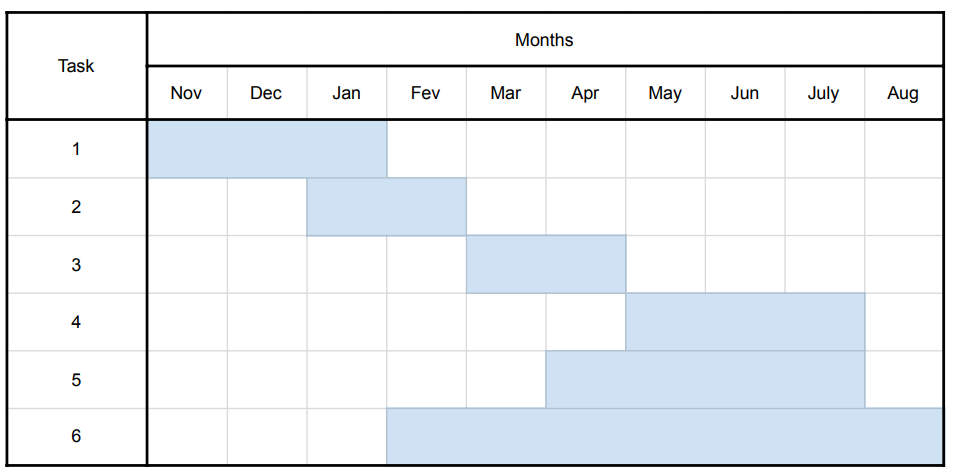
\includegraphics[width=0.85\linewidth]{gantt.png}
    \caption{Thesis project schedule}
    \label{fig:gantt}
\end{figure}